\documentclass[a4paper,12pt]{report}
\usepackage{graphicx}
\usepackage{fancyhdr}
\usepackage[absolute,overlay]{textpos}
\usepackage{lipsum}
\usepackage{tikz}
\usepackage{setspace}
\usepackage{enumitem}
\usepackage{titlesec}
\usepackage{geometry}
\usepackage[utf8]{inputenc}
\usepackage[T1]{fontenc}
\usepackage[french]{babel}
\usepackage{pgfgantt}
\usepackage[hidelinks]{hyperref}
\usepackage{caption}
\usepackage{float}
\usepackage{amsmath}
\usepackage{tocloft}
\usepackage{afterpage}
\usepackage{lscape}
\usepackage{titletoc}
\usepackage{cite}   
\usepackage{newunicodechar}
\usepackage{array}
\usepackage{tabularx}
\newunicodechar{’}{'}
\newunicodechar{‘}{'}
\newunicodechar{–}{--}
\newunicodechar{—}{---}
\newunicodechar{“}{``}
\newunicodechar{”}{''}
\newunicodechar{…}{\ldots{}}  % For better citation management
\setcounter{tocdepth}{3}
\setcounter{secnumdepth}{3}

\titlecontents{chapter}
  [0em] % left margin
  {\normalfont\bfseries} % above code
  {Chapitre~\thecontentslabel:\ } % numbered entry format
  {} % numberless entry format
  {\titlerule*[8pt]{.}\contentspage} % page format

  \renewcommand{\listfigurename}{Liste des Figures}
  \renewcommand{\cftfigpresnum}{Figure~}
  \renewcommand{\cftfigaftersnum}{.\ }
  \renewcommand{\cftfignumwidth}{4em} % Largeur pour le numéro de figure
  \renewcommand{\cftfigindent}{0em} % Pas d'indentation
  \renewcommand{\cftfigafterpnum}{\hspace{1em}} % Espacement après le numéro de page


  \titlecontents{figure}
  [0em] % left margin
  {\normalfont} % above code
  {Figure~\thecontentslabel:\ } % numbered entry format
  {} % numberless entry format
  {\titlerule*[8pt]{.}\contentspage} % page format
  \titlecontents{table}
  [0em] % left margin
  {\normalfont} % above code
  {Tableau~\thecontentslabel:\ } % numbered entry format
  {} % numberless entry format
  {\titlerule*[8pt]{.}\contentspage} % page format

  \renewcommand{\listtablename}{Liste des Tableaux}

\renewcommand{\cfttabpresnum}{Tableau~}
\renewcommand{\cfttabaftersnum}{.\ }
\renewcommand{\cfttabnumwidth}{6em} % Width for table number
\renewcommand{\cfttabindent}{0em} % No indentation
\renewcommand{\cfttabafterpnum}{\hspace{1em}} % Space after page number

% Configure the fancyhdr package
\fancypagestyle{plain}{
    \fancyhf{}
    \fancyhfoffset[L]{1cm}
    \fancyhfoffset[R]{1cm}
    \fancyhead[L]{
\includegraphics[width=5cm]{./logos/emsi.png}}
    \fancyhead[R]{\small \textit{\leftmark}} % Chapter name on the right
    \fancyfoot[C]{\thepage}
    \setlength{\headheight}{1.5cm}
    \setlength{\topmargin}{-1in}
    \setlength{\headsep}{3cm}
}

\pagestyle{fancy}
\fancyhf{}
\fancyhfoffset[L]{1cm}
\fancyhfoffset[R]{1cm}
\fancyhead[L]{
\includegraphics[width=5cm]{./logos/emsi.png}}
\fancyhead[R]{\small \textit{\leftmark}}
\fancyfoot[C]{\thepage}
\setlength{\headheight}{1.5cm}
\setlength{\topmargin}{-1in}
\setlength{\headsep}{3cm}

\begin{document}

% Title Page
% Title Page
\begin{titlepage}
% Background Images
\begin{tikzpicture}[remember picture, overlay]
\node[anchor=north west, xshift=-1cm, yshift=1cm] at (current page.north west) {
\includegraphics[width=4.5cm]{./logos/coin haut.png}};
\node[anchor=south east, xshift=0.2cm, yshift=-0.12cm] at (current page.south east) {
\includegraphics[width=4.5cm]{./logos/coin bas.png}};
\end{tikzpicture}

```
% Logos
\begin{textblock*}{3cm}(15cm,1cm)
    
\includegraphics[width=4.5cm]{./logos/logo.png}
\end{textblock*}

\begin{textblock*}{7cm}(3cm,1.2cm)
    
\includegraphics[width=4.5cm]{./logos/emsi.png}
\end{textblock*}

\begin{center}
    \vspace*{2.2cm}

    \textsc{\LARGE ÉCOLE MAROCAINE DES SCIENCES D'INGÉNIEUR}\\[0.25cm]
    
    \textsc{\Large PROJET DE FIN D'ÉTUDES}\\[0.35cm]

    \textsc{\Large Filière}\\[0.15cm]
    \textbf{\large Ingénierie Informatique et Réseaux}\\[0.15cm]
    \textbf{\large 5IIR -- 3\textsuperscript{ème} année du cycle ingénieur}\\[0.7cm]
    
    \fbox{
        \begin{minipage}{0.9\textwidth}
            \vspace{0.25cm}
            \centering
            \textbf{\Huge FinderrLink}\\[0.25cm]
            \textbf{\Large Conception et développement full-stack d'une plateforme de mise en relation entre freelances, entreprises et agences}
            \vspace{0.25cm}
        \end{minipage}
    }\\[0.8cm]

    \large \textbf{Réalisé par}\\[0.15cm]
    Afaki Abdelmajid\\[0.9cm]
    
    \begin{minipage}[t]{0.48\textwidth}
        \centering
        \large \textbf{Tuteur dans l'entreprise}\\[0.25cm]
        M. Reda Alami\\
        MEDIASSIVE
    \end{minipage}
    \hfill
    \begin{minipage}[t]{0.48\textwidth}
        \centering
        \large \textbf{Membres du jury}\\[0.25cm]
        M. / Mme ................................\\[0.15cm]
        M. / Mme ................................\\[0.15cm]
        M. / Mme ................................
    \end{minipage}

    \vspace*{1.2cm}

    \textbf{Durée du stage :} Février 2026 -- Juin 2026\\[0.25cm]
    \textbf{Année Universitaire 2025-2026}
    
\end{center}
```

\end{titlepage}

\clearpage

% Blank page between title page and Remerciements
\mbox{}
\clearpage

% Resetting to fancy after title page
\pagestyle{fancy}

% Sections
\markboth{\MakeUppercase{Remerciements}}{}
\section*{\Huge Remerciements}

\vspace{0.7cm}

\begin{spacing}{1.35}
Je tiens tout d’abord à exprimer ma profonde gratitude à mes parents, pour leur soutien permanent, leurs encouragements et leur confiance tout au long de mon parcours académique. Leur présence, leurs sacrifices et leur accompagnement ont constitué une source essentielle de motivation durant la réalisation de ce Projet de Fin d’Études.

Je souhaite également remercier mes amis et mes proches pour leur soutien moral, leurs conseils et leurs encouragements, qui m’ont aidé à avancer avec sérieux et détermination tout au long de cette expérience.

J’adresse mes sincères remerciements à M. Reda Alami, CEO de MEDIASSIVE et tuteur au sein de l’entreprise, pour son encadrement, sa disponibilité, ses orientations pertinentes et la confiance qu’il m’a accordée durant la réalisation de ce projet. Ses conseils ont grandement contribué à l’avancement et à la réussite du projet FinderrLink.

Je remercie également Mme Chaimae Mezouri, Développeuse IA, pour son accompagnement et ses échanges autour des aspects liés à l’intelligence artificielle du projet, ainsi que M. Noeam El Afia, UI/UX Designer, pour sa contribution à la réflexion autour de l’expérience utilisateur et de l’interface graphique.

Enfin, je tiens à remercier l’ensemble de mes enseignants ainsi que l’École Marocaine des Sciences de l’Ingénieur pour la qualité de la formation reçue, l’accompagnement pédagogique et les connaissances acquises tout au long de mon cursus. Ces acquis m’ont permis de mener à bien ce projet dans un cadre professionnel, technique et méthodologique.
\end{spacing}

\addcontentsline{toc}{chapter}{Remerciements}
\newpage
\markboth{\MakeUppercase{resume}}{}
\section*{\Huge Résumé}

\vspace{0.7cm}

\begin{spacing}{1.25}
Ce rapport présente le travail réalisé dans le cadre de mon Projet de Fin d’Études, portant sur la conception, le développement et le déploiement de FinderrLink, une plateforme web de mise en relation entre freelances, entreprises et agences. Le projet vise à faciliter la recherche de missions, la gestion des profils professionnels, le suivi des candidatures et la communication entre les différents acteurs de la plateforme.

FinderrLink repose sur une architecture full-stack moderne composée d’un frontend dynamique, d’un backend structuré et d’une base de données relationnelle. La plateforme intègre plusieurs modules fonctionnels, notamment la gestion des utilisateurs, des profils freelances, des missions, des candidatures, de la messagerie, des notifications, des tableaux de bord et d’un assistant intelligent destiné à améliorer l’expérience utilisateur.

Un élément important du projet est la mise en place d’un système RBAC, ou Role-Based Access Control, permettant de gérer les droits d’accès selon le rôle de chaque utilisateur. Les freelances, les entreprises, les agences et les administrateurs disposent ainsi d’interfaces, de permissions et de fonctionnalités adaptées à leurs besoins. Ce système permet d’assurer une meilleure sécurité, une séparation claire des responsabilités et une gestion cohérente des accès.

Le projet couvre également la phase de déploiement dans un environnement serveur, incluant la configuration des services applicatifs, la gestion de la base de données, la mise en place du reverse proxy, la sécurisation des accès et la préparation de l’application pour une utilisation en production.
\end{spacing}

\vspace{0.4cm}
\noindent \textbf{Mots clés :} FinderrLink, Développement full-stack, Déploiement web, Plateforme web, Freelance, Entreprise, Agence, RBAC, Missions, Candidatures, Messagerie, Notifications, Intelligence artificielle, API, Base de données.

\addcontentsline{toc}{chapter}{Résumé}
\newpage\markboth{\MakeUppercase{Absract}}{}
\section*{\Huge Abstract}

\vspace{0.7cm}

\begin{spacing}{1.25}
This report presents the work carried out as part of my Final Year Project, focusing on the design, development, and deployment of FinderrLink, a web platform dedicated to connecting freelancers, companies, and agencies. The project aims to facilitate mission search, professional profile management, application tracking, and communication between the different users of the platform.

FinderrLink is based on a modern full-stack architecture composed of a dynamic frontend, a structured backend, and a relational database. The platform includes several functional modules such as user management, freelancer profiles, mission management, applications, messaging, notifications, dashboards, and an intelligent assistant designed to improve the user experience.

An important aspect of the project is the implementation of an RBAC system, or Role-Based Access Control, which manages access rights according to each user’s role. Freelancers, companies, agencies, and administrators each have specific interfaces, permissions, and features adapted to their needs. This system improves security, ensures a clear separation of responsibilities, and provides consistent access management across the application.

The project also covers the deployment phase in a server environment, including application service configuration, database management, reverse proxy setup, access security, and preparation of the platform for production use.
\end{spacing}

\vspace{0.4cm}
\noindent \textbf{Keywords:} FinderrLink, Full-stack development, Web deployment, Web platform, Freelancer, Company, Agency, RBAC, Missions, Applications, Messaging, Notifications, Artificial intelligence, API, Database.

\addcontentsline{toc}{chapter}{Absract}
\newpage

% Table of Contents
\cleardoublepage
\pagestyle{plain}
\newpage
\addcontentsline{toc}{chapter}{Table des matières}
\tableofcontents

\newpage
\addcontentsline{toc}{chapter}{Liste des Figures}
\listoffigures

\newpage
\addcontentsline{toc}{chapter}{Liste des Tableaux}
\listoftables

\newpage

% Main Content
\pagestyle{fancy}
\addcontentsline{toc}{chapter}{Introduction Générale}
\markboth{\MakeUppercase{Introduction Générale}}{}
\chapter*{Introduction générale}


Dans le cadre de mon Projet de Fin d’Études au sein de MEDIASSIVE, entreprise basée à Tanger et spécialisée dans le développement digital, les solutions web et l’innovation technologique, j’ai travaillé sur la conception, le développement et le déploiement d’une plateforme web nommée FinderrLink. Ce projet s’inscrit dans la vision de MEDIASSIVE, qui vise non seulement à proposer des services digitaux, mais aussi à lancer ses propres solutions SaaS internes répondant à des besoins réels du marché.

FinderrLink est une plateforme de mise en relation entre freelances, entreprises et agences. Elle permet de centraliser la gestion des profils professionnels, des missions, des candidatures, de la messagerie, des notifications et des tableaux de bord dans un seul environnement numérique. Elle vise ainsi à simplifier la recherche de talents, la publication des missions et le suivi des collaborations professionnelles.

Durant ce projet, j’ai occupé le rôle de chef d’équipe, ce qui m’a permis de participer aux aspects techniques et organisationnels. Mon intervention a porté sur l’analyse des besoins, la conception de l’architecture, le développement full-stack, la mise en place du système RBAC, la coordination des tâches et la préparation du déploiement. Le système RBAC permet de gérer les droits d’accès selon les rôles : freelance, entreprise, agence et administrateur \cite{owasp}.

Le développement de FinderrLink a présenté plusieurs défis, notamment la gestion de rôles différents, la structuration de la base de données, le suivi des candidatures, l’intégration de la messagerie, la mise en place des notifications et le déploiement dans un environnement serveur. Une particularité importante du projet réside dans le rôle hybride de l’agence, qui peut publier des missions comme une entreprise et postuler à des missions comme un freelance.

Ce projet m’a permis de renforcer mes compétences en développement web full-stack, en conception logicielle, en sécurité applicative, en gestion de base de données, en déploiement et en coordination d’équipe. Le présent rapport présente l’entreprise d’accueil, le contexte du projet, l’analyse des besoins, la conception, les technologies utilisées, la réalisation des modules, le déploiement, les tests et les perspectives d’amélioration de FinderrLink.


\newpage

\markboth{\MakeUppercase{Présentation de l'Entreprise}}{}
\chapter{Présentation de l'Entreprise}

\section{Introduction}

Dans un contexte marqué par la transformation numérique et l'émergence des technologies Web3, les entreprises se tournent vers des solutions innovantes pour renforcer leur présence digitale et améliorer leur compétitivité. Mediassive s'inscrit dans cette dynamique en tant qu'agence spécialisée en marketing digital et Web3, offrant un accompagnement stratégique et technologique aux entreprises souhaitant évoluer dans l'univers du numérique.

\section{Description de l'Activité de l'Entreprise et de ses Produits}

\subsection{Fiche Technique}

\begin{table}[H]
    \centering
    \begin{tabular}{|l|l|}
    \hline
    \textbf{Dénomination} & Mediassive SARL (société à responsabilité limitée unipersonnelle) \\
    \hline
    \textbf{Siège social} & Lot 1500 Hay Hajari N°10, Laâyoune – Maroc \\
    \hline
    \textbf{Capital social} & 100 000 MAD \\
    \hline
    \textbf{Secteur d'activité} & Marketing digital, Web3, services informatiques et technologiques \\
    \hline
    \textbf{Dirigeant} & Reda Alamikasri \\
    \hline
    \textbf{Site officiel} & www.mediassive.com \\
    \hline
    \end{tabular}
    
    \caption{Fiche signalétique de Mediassive}
    \label{tab:fichesignaletique}
    \end{table}

\subsection{Taille et Effectif}

Mediassive compte une équipe jeune, dynamique et pluridisciplinaire.

\textbf{Effectif estimé :} Entre 10 et 20 collaborateurs

\textbf{Domaines de compétence :} Développement informatique, gestion de projets, marketing digital, design, community management, blockchain et crypto-actifs.

\section{Historique de l'Entreprise}

Fondée il y a plus de 6 ans, Mediassive a d'abord démarré en tant qu'agence de marketing digital classique, avant de se spécialiser progressivement dans les technologies Web3. L'entreprise a accompagné plusieurs projets innovants tels que Tikeey (billetterie blockchain), Doc Minter (authentification de documents), et Exclusive Beats (NFT musicaux). Cette évolution illustre sa volonté d'être un acteur majeur de la transition numérique au Maroc et à l'international.

\section{Organisation Interne de l'Entreprise}

\subsection{Organigramme Commenté}

\begin{figure}[H]
    \centering
    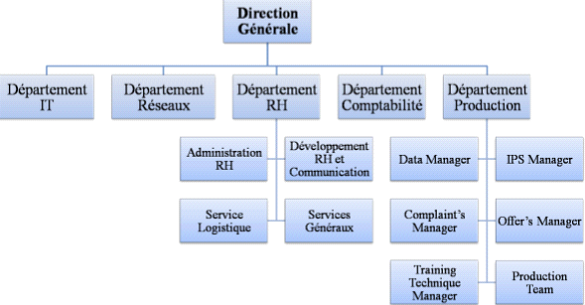
\includegraphics[width=0.8\textwidth]{./figures/Organigrammecmh.png}
    \caption{Organigramme de Mediassive}
    \label{fig:organigramme}
    \end{figure}
    
L'organisation de Mediassive repose sur une structure hiérarchique simple et efficace. La Direction Générale supervise la stratégie et les opérations de l'entreprise. Le Pôle IT \& Développement s'occupe du développement Web, mobile, blockchain et de la maintenance technique. Le Pôle Marketing Digital gère le SEO, les campagnes publicitaires, la gestion des réseaux sociaux et la stratégie de contenu. Le Pôle Design \& Communication se charge de l'identité visuelle, du UX/UI design et des supports multimédias. Enfin, le Support \& Assistance Client assure la relation client, le helpdesk et le suivi des projets.

\subsection{Services au Sein de l'Entreprise}

Mediassive propose une gamme complète de services incluant le marketing digital avec SEO, SEA et social media management. L'entreprise excelle également dans le développement Web et Mobile, ainsi que dans les solutions Web3 innovantes comprenant la blockchain, les smart contracts, les NFT et les dApps. Le design graphique et le branding font également partie de ses compétences, tout comme le consulting et la formation en stratégie digitale.

\section{Environnement de l'Entreprise}

\subsection{Clientèle}

La clientèle de Mediassive est variée et comprend principalement des startups technologiques, des entreprises locales souhaitant renforcer leur visibilité digitale, ainsi que des projets internationaux liés à la blockchain et au Web3.

\subsection{Fournisseurs}

L'entreprise collabore avec des fournisseurs de solutions numériques (hébergement cloud, outils analytiques, régies publicitaires en ligne, plateformes de développement).

\subsection{Concurrence}

Mediassive évolue dans un secteur compétitif où l'on retrouve des agences locales de communication digitale et des agences spécialisées en Web3 à l'international. Son atout réside dans son double positionnement : marketing digital classique et solutions Web3 innovantes.

\section{Présentation de l'Entreprise d'Accueil}

\subsection{À Propos de l'Entreprise}

Mediassive est une agence qui combine créativité, expertise digitale et technologies émergentes pour accompagner les entreprises dans leur développement numérique.

\subsection{Vision et Objectifs}

Mediassive aspire à être un acteur de référence dans le marketing digital et Web3 au Maroc et à l'échelle internationale. L'entreprise s'engage à promouvoir l'adoption des solutions blockchain et décentralisées, tout en contribuant activement à la digitalisation des entreprises locales.

\subsection{Locaux et Implantation}

L'entreprise est implantée à Laâyoune avec une présence au Technopark de Tanger, un espace favorisant l'innovation et la collaboration.
\section{Contexte et problématique}

\subsection{Contexte général}

Le marché du travail connaît aujourd’hui une transformation importante, marquée par le développement du freelancing, du travail à distance et des collaborations flexibles entre professionnels indépendants, entreprises et agences. Les organisations recherchent de plus en plus des profils qualifiés capables d’intervenir rapidement sur des missions spécifiques, tandis que les freelances souhaitent accéder à des opportunités adaptées à leurs compétences, à leur disponibilité, à leur localisation et à leurs préférences professionnelles.

Dans ce contexte, les plateformes de mise en relation jouent un rôle essentiel. Elles permettent de rapprocher les besoins des entreprises et des agences avec les compétences disponibles sur le marché. Cependant, les solutions existantes restent souvent limitées à une simple publication d’offres ou à une recherche manuelle de profils. Cette approche rend le processus parfois long, peu structuré et difficile à suivre.

FinderrLink s’inscrit dans cette logique de transformation digitale en proposant une plateforme web centralisée permettant de gérer les profils, les missions, les candidatures, les échanges, les notifications et les tableaux de bord. L’objectif est de faciliter la collaboration entre les différents acteurs tout en assurant une gestion claire des rôles et des permissions.

\subsection{Présentation des acteurs de la plateforme}

La plateforme FinderrLink repose sur plusieurs types d’utilisateurs ayant chacun des besoins et des droits spécifiques. Le freelance peut créer et gérer son profil professionnel, consulter les missions disponibles, postuler aux opportunités qui correspondent à son profil, sauvegarder des missions et suivre l’état de ses candidatures.

L’entreprise représente principalement un recruteur direct. Elle peut créer et publier des missions, gérer les candidatures reçues, consulter les profils freelances, sauvegarder des talents et entrer en contact avec les profils correspondant à ses besoins. Son rôle est donc orienté vers la recherche de compétences et la gestion des missions qu’elle propose.

L’agence possède un rôle plus flexible. Elle peut créer et gérer ses propres missions, comme une entreprise, mais elle peut également consulter les missions disponibles et y postuler, de manière similaire à un freelance. Cette particularité permet à l’agence d’agir à la fois comme recruteur pour ses propres besoins ou ceux de ses clients, et comme prestataire capable de répondre à des missions publiées sur la plateforme.

L’administrateur dispose d’un rôle de supervision. Il peut suivre l’activité globale de la plateforme, gérer les utilisateurs, contrôler les données principales et assurer le bon fonctionnement du système.

\subsection{Problématique de la fragmentation des informations}

L’un des principaux problèmes rencontrés dans le domaine du freelancing est la dispersion des informations. Les profils, les missions, les candidatures, les messages et les notifications sont souvent gérés à travers plusieurs outils ou plateformes distinctes. Cette fragmentation complique le suivi des activités, augmente le risque de perte d’information et ralentit les processus de recrutement et de collaboration.

Pour les freelances, cette situation rend la recherche de missions plus longue et moins efficace, car les opportunités ne sont pas toujours bien structurées ou adaptées à leur profil. Pour les entreprises, elle complique l’identification rapide des talents pertinents. Pour les agences, qui peuvent à la fois recruter et postuler à des missions, le besoin d’une gestion centralisée devient encore plus important.

Il est donc nécessaire de proposer une solution capable de regrouper l’ensemble des informations dans un environnement unique, clair et organisé.

\subsection{Problématique de la gestion des rôles et des accès}

Dans une plateforme regroupant plusieurs types d’utilisateurs, la gestion des droits d’accès constitue un enjeu essentiel. Les fonctionnalités accessibles ne doivent pas être identiques pour tous les utilisateurs. Un freelance ne doit pas avoir les mêmes permissions qu’une entreprise, une entreprise ne doit pas avoir les mêmes droits qu’une agence, et l’administrateur doit disposer d’un niveau d’accès plus avancé.

Cette diversité des rôles impose la mise en place d’un système RBAC, ou Role-Based Access Control. Ce système permet d’attribuer des permissions précises selon le rôle de chaque utilisateur. Il garantit que chaque acteur accède uniquement aux fonctionnalités qui correspondent à ses responsabilités.

Dans FinderrLink, cette logique est particulièrement importante, car l’agence possède un rôle hybride. Elle peut publier des missions comme une entreprise, mais elle peut également postuler à des missions comme un freelance. Le système de gestion des rôles doit donc être suffisamment précis pour prendre en charge ces différences fonctionnelles tout en maintenant la sécurité et la cohérence de l’application.

\subsection{Problématique du suivi des candidatures et de la communication}

Le suivi des candidatures représente un autre défi important. Les freelances ont besoin de connaître l’état de leurs candidatures, tandis que les entreprises et les agences doivent pouvoir organiser, analyser et traiter les candidatures reçues. Sans un outil structuré, ce suivi peut rapidement devenir complexe, surtout lorsque plusieurs missions et plusieurs profils sont gérés en même temps.

La communication entre les utilisateurs doit également être encadrée. Les échanges doivent respecter les règles métiers de la plateforme afin d’éviter les interactions non pertinentes ou non autorisées. La messagerie, les notifications et les statuts de candidature deviennent donc des éléments essentiels pour assurer une collaboration fluide et organisée entre les différents acteurs.

\subsection{Problématique liée à l’aide à la décision}

Un autre besoin important concerne l’aide à la décision. Les freelances peuvent avoir des difficultés à identifier les missions les plus adaptées à leur profil, surtout lorsque plusieurs opportunités semblent similaires. Les entreprises et les agences, de leur côté, peuvent rencontrer des difficultés à trouver rapidement les profils les plus pertinents parmi un grand nombre de freelances.

L’intégration d’un assistant intelligent permet de répondre à ce besoin en aidant les utilisateurs à rechercher des missions, comparer des opportunités, comprendre les détails d’une offre ou mieux exploiter les informations disponibles sur la plateforme. Cette dimension intelligente améliore l’expérience utilisateur et rend la plateforme plus efficace.

\subsection{Problème identifié}

Face à ces constats, le problème central peut être formulé ainsi :

\textbf{L’absence d’une plateforme centralisée, sécurisée et intelligente pour gérer la mise en relation entre freelances, entreprises et agences constitue un frein à l’efficacité du recrutement, au suivi des missions, à la gestion des candidatures et à la collaboration professionnelle.}

Une telle solution doit permettre de regrouper les profils, les missions, les candidatures, les échanges, les notifications et les tableaux de bord dans un seul environnement. Elle doit également intégrer une gestion précise des rôles, notamment pour distinguer les permissions du freelance, de l’entreprise, de l’agence et de l’administrateur.

Ainsi, FinderrLink vise à répondre à cette problématique en proposant une plateforme web complète, structurée et évolutive, capable d’améliorer la mise en relation entre les différents acteurs et de simplifier la gestion des processus liés aux missions professionnelles.
\section{Conclusion}

En conclusion, ce chapitre a permis de présenter le contexte général du projet FinderrLink, sa problématique ainsi que les objectifs visés. Le projet répond à un besoin réel de centralisation, de sécurité et d’efficacité dans la mise en relation entre freelances, entreprises et agences. Il s’inscrit également dans la vision de MEDIASSIVE, qui ne se limite pas aux services digitaux classiques, mais ambitionne aussi de développer et lancer ses propres solutions SaaS internes afin de répondre à des problématiques concrètes du marché.

\newpage
\markboth{\MakeUppercase{Département d'Attache}}{}
\chapter{Département d'attache et mission}

\section{Introduction}

Ce chapitre présente le département d’attache au sein de MEDIASSIVE ainsi que les missions qui m’ont été confiées durant mon Projet de Fin d’Études. Il met l’accent sur mon rôle en tant que chef d’équipe stagiaire, développeur full-stack et responsable du déploiement, ainsi que sur ma participation à plusieurs projets internes de l’entreprise, notamment FinderrLink, ScanVivo et Batiscan.

\section{Aperçu sur le département d'attache}

Le département développement web et digital de MEDIASSIVE constitue le pôle technique chargé de concevoir, développer, déployer et maintenir des solutions numériques. Il intervient aussi bien sur des projets clients que sur des projets internes de type SaaS, dans une logique d’innovation et de création de valeur pour l’entreprise.

Le travail au sein de ce département suit généralement plusieurs étapes : analyse des besoins, conception de l’architecture, développement front-end et back-end, intégration de la base de données, tests, correction des anomalies, déploiement et suivi technique. Ces étapes nécessitent une collaboration entre plusieurs profils, notamment les développeurs full-stack, les développeurs IA, les designers UI/UX et les responsables de projet.

\section{Position et rôle dans l'entreprise}

Durant mon stage, j’ai occupé le rôle de chef d’équipe stagiaire au sein du département digital. Mon poste ne se limitait pas uniquement au développement technique, mais comprenait également la coordination avec les autres stagiaires, le suivi de l’avancement des tâches, l’organisation du travail et la vérification de la cohérence entre les différentes parties des projets.

Sur le projet FinderrLink, j’ai principalement travaillé en tant que développeur full-stack et responsable du déploiement. Mes missions ont porté sur la mise en place de la base technique de la plateforme, le développement des premières fonctionnalités, la structuration de l’application, la gestion des rôles et la préparation de l’environnement de déploiement. Les détails fonctionnels de FinderrLink seront présentés dans les chapitres suivants.

L’équipe principale de FinderrLink était composée de plusieurs profils complémentaires. J’ai assuré la partie développement full-stack et déploiement, Mme Chaimae Mezouri a travaillé sur la partie intelligence artificielle, et M. Noeam El Afia a participé à la conception UI/UX de la plateforme. Cette organisation a permis de répartir les tâches selon les compétences de chaque membre.

\section{Organisation des projets et coordination}

En plus de FinderrLink, j’ai également participé aux projets ScanVivo et Batiscan. Dans un premier temps, j’ai développé et déployé les premières versions basiques de ces deux plateformes afin de mettre en place une base fonctionnelle exploitable. Par la suite, ces projets ont été confiés à une équipe de stagiaires à distance, chargée de poursuivre leur développement sous suivi et orientation.

Une autre équipe de stagiaires à distance a été dédiée au développement d’un panneau d’administration pour FinderrLink. Ce panneau avait pour objectif de permettre la supervision de l’application, notamment à travers le suivi des utilisateurs, des missions et des données principales de la plateforme.

Mon rôle consistait à coordonner ces équipes, suivre l’avancement des tâches, expliquer les besoins, orienter les choix techniques et vérifier que le travail réalisé restait cohérent avec les objectifs des projets. Cette organisation m’a permis de développer des compétences en gestion d’équipe, en communication et en suivi de projet, en plus de mes compétences techniques.

\section{Tâches réalisées}

Les principales tâches réalisées durant cette mission peuvent être résumées comme suit :

\begin{itemize}
\item Développement full-stack de la première version de FinderrLink.
\item Préparation et réalisation du déploiement de la plateforme.
\item Mise en place des bases techniques des projets ScanVivo et Batiscan.
\item Déploiement des premières versions basiques de ScanVivo et Batiscan.
\item Coordination avec l’équipe IA et l’équipe UI/UX.
\item Suivi de deux équipes de stagiaires à distance.
\item Accompagnement des stagiaires dans la compréhension des besoins.
\item Suivi du développement du panneau d’administration de FinderrLink.
\item Vérification de la cohérence technique et fonctionnelle entre les projets.
\end{itemize}

\section{Conclusion}

Cette mission m’a permis de participer à plusieurs projets numériques au sein de MEDIASSIVE, tout en occupant un rôle à la fois technique et organisationnel. À travers FinderrLink, ScanVivo et Batiscan, j’ai pu renforcer mes compétences en développement full-stack, en déploiement web et en coordination d’équipe. Cette expérience m’a également permis de mieux comprendre le fonctionnement d’un environnement professionnel orienté vers la création de solutions SaaS internes et la gestion de projets digitaux.




\markboth{\MakeUppercase{Étude bibliographique}}{}
\chapter{Étude bibliographique}

\section{Introduction}

Dans un monde numérique en constante évolution, les données sont devenues le \textit{pétrole du XXIe siècle}. Les entreprises, quelle que soit leur taille, s’appuient de plus en plus sur l’analytique pour prendre des décisions stratégiques éclairées. La capacité à \textbf{collecter, traiter, visualiser et interpréter les indicateurs clés de performance (KPI)} est devenue essentielle pour rester compétitif dans des secteurs tels que le marketing digital, le commerce électronique et la communication en ligne.

Cependant, cette transformation s’accompagne de défis majeurs : la \textbf{dispersion des sources de données}, la \textbf{complexité technique des intégrations} et la difficulté pour des utilisateurs non spécialisés de tirer profit d’outils parfois conçus pour des experts.

Le projet \textbf{Mediassive Analytics} s’inscrit dans ce contexte en proposant une solution innovante, centrée sur la \textbf{centralisation des données}, la \textbf{simplicité d’utilisation} et l’\textbf{adaptabilité aux besoins spécifiques} d’une agence digitale et de ses clients.

\section{Contexte et tendances actuelles}

\subsection{L’importance des données dans la prise de décision}
L’utilisation des données occupe désormais une place centrale dans la gouvernance des entreprises. Selon une étude de Gartner (2022)\cite{gartner2022}, plus de \textbf{70\% des entreprises} déclarent que leurs décisions stratégiques reposent principalement sur l’analyse de données. Pourtant, seules 30\% estiment exploiter pleinement leur potentiel analytique.

Les données ne se limitent pas à un rôle de reporting : elles constituent un véritable levier de croissance. En effet, elles permettent non seulement d’évaluer la performance passée mais aussi de guider les choix futurs. Parmi les principales applications, on retrouve :
\begin{itemize}
    \item l’identification des canaux les plus performants ;
    \item l’optimisation des budgets marketing en fonction du retour sur investissement (ROI) ;
    \item le suivi en temps réel de l’évolution des campagnes publicitaires.
\end{itemize}

\subsection{La démocratisation de l’analytique}
Autrefois réservés aux grandes entreprises disposant d’équipes spécialisées en business intelligence, les outils d’analytique se sont progressivement démocratisés. Désormais, même les PME et les start-ups ressentent le besoin de suivre précisément leurs KPI afin de rester compétitives.  
Cette tendance s’accompagne d’une exigence accrue : proposer des solutions qui soient \textbf{accessibles aux non-techniciens}, sans pour autant sacrifier la profondeur d’analyse.

\section{Analyse des solutions existantes}

L’offre actuelle en matière de solutions analytiques est riche et variée. Toutefois, chacune présente des atouts et des limites qui méritent d’être examinés.

\subsection{Tableaux de bord traditionnels}
Les outils tels que \textbf{Google Data Studio (Looker Studio)}\cite{lookerstudio}, \textbf{Tableau}\cite{tableau}, \textbf{Power BI}\cite{powerbi} ou encore \textbf{QlikView}\cite{qlik} dominent le marché des tableaux de bord classiques. Ils offrent une grande puissance d’analyse et disposent de connecteurs multiples pour intégrer différentes sources de données.

\textbf{Avantages :}
\begin{itemize}
    \item puissance analytique avancée ;
    \item connectivité avec un grand nombre de plateformes.
\end{itemize}

\textbf{Limites :}
\begin{itemize}
    \item complexité de configuration nécessitant une expertise technique ;
    \item coûts élevés, souvent difficiles à supporter pour une PME.
\end{itemize}

\subsection{Solutions marketing intégrées}
Certaines plateformes comme \textbf{HubSpot}\cite{hubspot}, \textbf{SEMrush}\cite{semrush} ou \textbf{Zoho Analytics}\cite{zoho} proposent des modules d’analytique directement intégrés à leurs services.

Ces solutions séduisent par leur simplicité et leur aspect « tout-en-un », mais elles enferment l’entreprise dans un écosystème propriétaire. Les coûts récurrents élevés et la flexibilité réduite représentent des freins à leur adoption pour certaines structures.

\subsection{Agrégateurs de données}
Des outils tels que \textbf{Supermetrics}\cite{supermetrics}, \textbf{Zapier}\cite{zapier} ou \textbf{Make (Integromat)}\cite{make} jouent un rôle d’intermédiaires en facilitant l’interconnexion entre plateformes hétérogènes.

Leur principal atout réside dans la simplification des flux de données. Toutefois, leur utilisation implique souvent des compétences techniques avancées et les coûts peuvent rapidement augmenter lorsqu’un grand nombre de connecteurs est requis.

\section{État de l’art des technologies utilisées}

\subsection{API et connecteurs}
Les API constituent la colonne vertébrale des intégrations multiplateformes. Elles permettent l’extraction en temps réel de données provenant de Google, Meta ou encore LinkedIn. Cependant, chaque API présente ses propres contraintes : limitations de quotas, changements fréquents dans les règles d’accès ou complexité de la documentation.

\subsection{Intelligence artificielle}
Au-delà du reporting descriptif, l’intelligence artificielle ouvre la voie à l’\textbf{analyse prédictive}. Elle rend possible des fonctionnalités innovantes telles que :
\begin{itemize}
    \item l’anticipation des performances d’une campagne ;
    \item la détection automatique d’anomalies dans les données ;
    \item la personnalisation des recommandations stratégiques.
\end{itemize}

\subsection{Visualisation interactive}
Les bibliothèques modernes comme \textbf{D3.js}\cite{d3}, \textbf{Plotly}\cite{plotly} ou \textbf{Chart.js}\cite{chartjs} offrent la possibilité de rendre les graphiques interactifs. Cela permet une exploration intuitive et dynamique des données, facilitant leur compréhension par des utilisateurs non spécialisés.

\section{Enjeux et défis actuels}

L’analyse bibliographique met en lumière plusieurs enjeux majeurs qui conditionnent le succès d’une solution analytique moderne. Ces enjeux peuvent être résumés ainsi :
\begin{enumerate}
    \item \textbf{Accessibilité} : rendre l’analytique exploitable par des non-experts.
    \item \textbf{Centralisation} : regrouper toutes les données en un seul endroit.
    \item \textbf{Coût} : adapter le modèle économique aux capacités financières des PME.
    \item \textbf{Sécurité et confidentialité} : respecter les réglementations telles que le RGPD.
    \item \textbf{Scalabilité} : permettre à l’outil de s’adapter à l’évolution des volumes de données.
\end{enumerate}

\section{Apports de Mediassive Analytics}

La solution proposée par \textbf{Mediassive Analytics} entend répondre directement aux limites identifiées dans les solutions existantes. Ses atouts principaux sont les suivants :
\begin{itemize}
    \item une \textbf{interface intuitive} pensée pour les non-techniciens ;
    \item la \textbf{centralisation des données} issues de multiples canaux en un seul tableau de bord ;
    \item une \textbf{personnalisation poussée} des KPI selon les besoins de chaque client ;
    \item une \textbf{évolutivité} grâce à l’intégration progressive de nouvelles sources ;
    \item une \textbf{accessibilité financière}, parfaitement adaptée aux agences digitales et PME.
\end{itemize}

\section{Comparatif avec les solutions existantes}

\begin{table}[H]
\centering
\setlength{\tabcolsep}{4pt}
\renewcommand{\arraystretch}{1.3}
\begin{tabular}{|p{3cm}|p{2.5cm}|p{2.5cm}|p{2.5cm}|p{2.5cm}|}
\hline
\textbf{Critère} & \textbf{Google Data Studio} & \textbf{Tableau / Power BI} & \textbf{HubSpot} & \textbf{Mediassive Analytics} \\ \hline
Simplicité d’utilisation & Moyenne & Faible & Bonne  & \textbf{Très bonne} \\ \hline
Coût & Gratuit / Premium & Élevé & Élevé  & \textbf{Accessible} \\ \hline
Intégration multiplateformes & Moyenne & Bonne & Limitée  & \textbf{Optimisée} \\ \hline
Personnalisation des KPI & Limitée & Bonne & Limitée  & \textbf{Très bonne} \\ \hline
\end{tabular}
\caption{Comparatif entre les solutions existantes et Mediassive Analytics}
\end{table}

\section{Perspectives futures}

À moyen terme, les solutions analytiques devront évoluer vers des fonctionnalités encore plus intelligentes et automatisées. Parmi les pistes prometteuses, on retrouve :
\begin{itemize}
    \item l’\textbf{automatisation avancée}, avec la génération de rapports et d’alertes intelligentes ;
    \item l’\textbf{analyse prédictive} renforcée par l’intelligence artificielle ;
    \item la \textbf{personnalisation dynamique}, permettant une adaptation du tableau de bord en fonction du profil utilisateur.
\end{itemize}

\section{Conclusion}

L’étude bibliographique montre que, malgré la richesse des solutions existantes, des limites persistent en termes de coût, d’accessibilité et de flexibilité.  

\textbf{Mediassive Analytics} se positionne comme une alternative crédible et innovante en combinant \textbf{simplicité d’utilisation}, \textbf{centralisation des données} et \textbf{personnalisation avancée}, ce qui en fait une solution adaptée aux besoins concrets des agences digitales et des PME.

\newpage

\markboth{\MakeUppercase{Conception de l'application}}{}
\numberwithin{figure}{section}

\chapter{Conception du systeme}

\section{Introduction}

Ce chapitre presente la conception du systeme FinderrLink. L'objectif est de donner une vision claire du fonctionnement general de la plateforme avant de passer a la realisation technique. Pour cela, trois diagrammes UML sont utilises : le diagramme de cas d'utilisation, le diagramme de classes et le diagramme de composants.

Le diagramme de cas d'utilisation permet de comprendre les interactions entre les acteurs et les principales fonctionnalites de la plateforme. Le diagramme de classes montre la structure interne du systeme a travers les entites principales et leurs relations. Enfin, le diagramme de composants presente l'organisation technique globale de l'application et les echanges entre ses differentes parties.

\section{Diagramme de cas d'utilisation}

Le diagramme de cas d'utilisation ci-dessous presente les principales actions possibles dans FinderrLink. Il permet de visualiser les roles des differents acteurs et les fonctionnalites accessibles selon chaque profil utilisateur.

\begin{figure}[H]
\centering
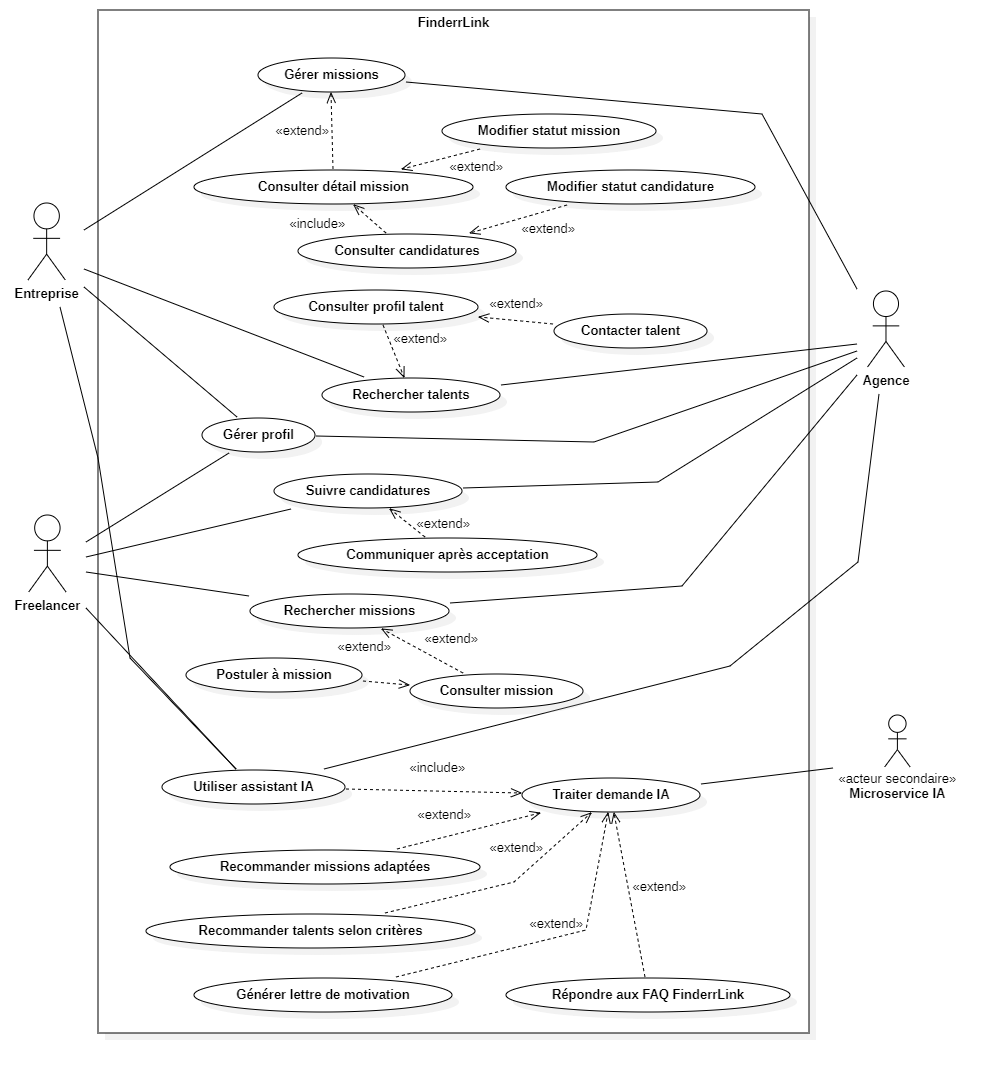
\includegraphics[width=0.95\textwidth]{./figures/UseCaseDiagram1.png}
\caption{Diagramme de cas d'utilisation - FinderrLink}
\label{fig:usecase_diagram_finderrlink}
\end{figure}

\subsection{Explication du diagramme de cas d'utilisation}

Le rectangle represente le systeme FinderrLink. Les acteurs places a l'exterieur du rectangle representent les utilisateurs ou services qui interagissent avec la plateforme. Les ovales representent les fonctionnalites principales.

Le freelance peut rechercher des missions, consulter une mission, postuler, suivre ses candidatures et communiquer apres acceptation. L'entreprise peut gerer ses missions, consulter les candidatures, modifier leur statut, rechercher des talents et contacter un talent. L'agence possede un role particulier, car elle peut publier des missions comme une entreprise et postuler a des missions comme un freelance.

Les relations \texttt{<<include>>} indiquent qu'une action contient obligatoirement une autre action. Les relations \texttt{<<extend>>} indiquent qu'une action peut completer une autre action selon le contexte. Par exemple, utiliser l'assistant IA inclut le traitement de la demande IA, tandis que recommander des missions adaptees ou generer une lettre de motivation sont des extensions possibles du traitement IA.

\section{Diagramme de classes UML}

Le diagramme de classes ci-dessous represente la structure principale de FinderrLink. Il montre les entites importantes du systeme, notamment les utilisateurs, les missions, les candidatures, les conversations, les notifications, les categories et la partie liee a l'assistant IA.

\begin{figure}[H]
\centering
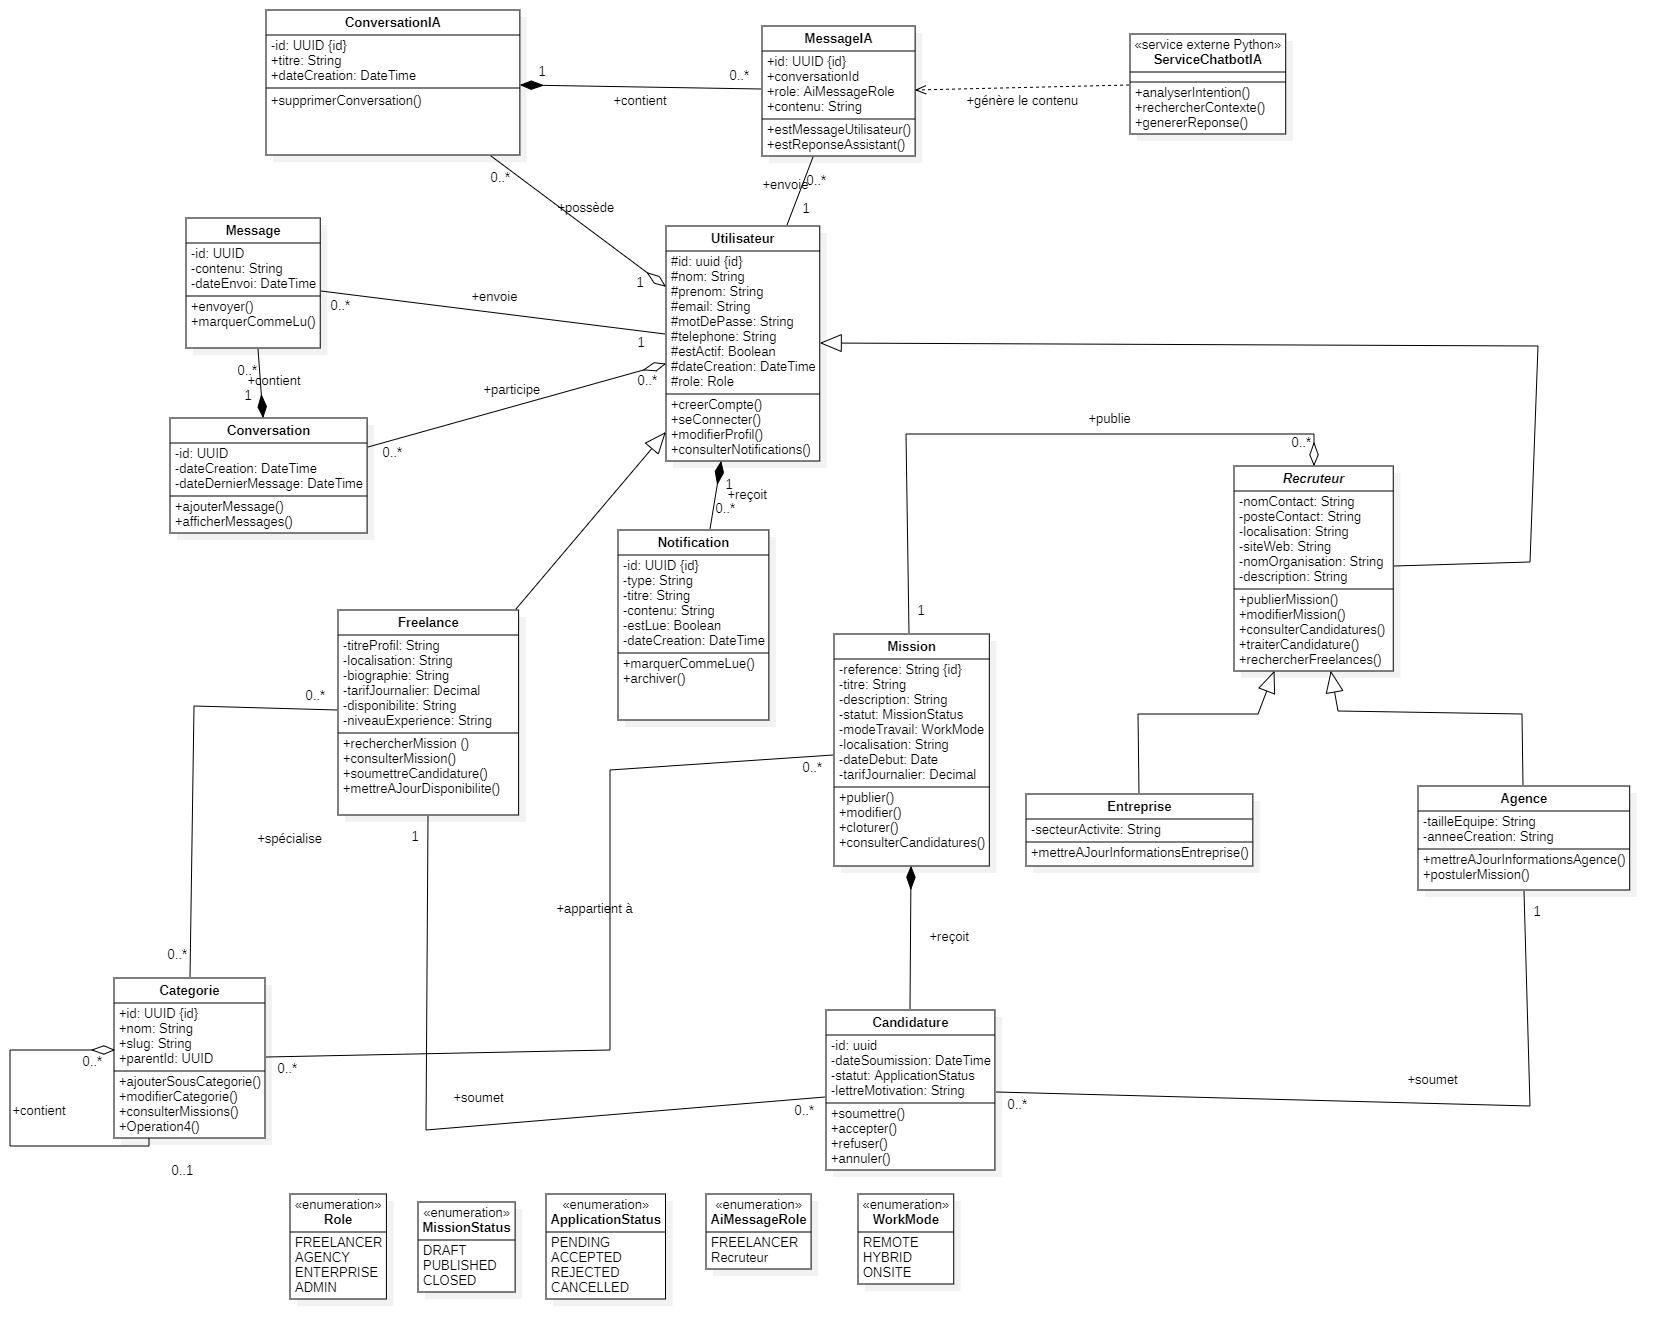
\includegraphics[width=1\textwidth]{./figures/ClassDiagram1.png}
\caption{Diagramme de classes UML - FinderrLink}
\label{fig:class_diagram_finderrlink}
\end{figure}

\subsection{Cle de lecture du diagramme de classes}

Une classe UML est representee par un rectangle divise en trois parties : le nom de la classe, les attributs et les methodes. Les attributs representent les donnees stockees, tandis que les methodes representent les actions possibles.

Le symbole \textbf{+} indique un element public. Le symbole \textbf{-} indique un element prive. Le symbole \textbf{\#} indique un element protege. Ces symboles permettent de preciser le niveau d'acces aux donnees et aux methodes.

L'heritage permet de representer une specialisation. Dans ce diagramme, les classes \textbf{Freelance}, \textbf{Recruteur}, \textbf{Entreprise} et \textbf{Agence} sont liees a la classe \textbf{Utilisateur}. Cela signifie que ces classes partagent des informations communes, comme le nom, l'email, le mot de passe, le telephone et le role.

L'agregation represente une relation souple entre deux classes. Les objets peuvent exister separement. La composition represente une relation plus forte, ou un element depend directement d'un autre. Par exemple, une conversation contient des messages, et une mission peut etre liee a plusieurs candidatures.

Les enumerations representent des listes de valeurs fixes. Elles permettent d'eviter les valeurs incoherentes. Par exemple, \textbf{Role} definit les types d'utilisateurs, \textbf{MissionStatus} definit l'etat d'une mission, \textbf{ApplicationStatus} definit le statut d'une candidature, et \textbf{WorkMode} definit le mode de travail.

\subsection{Explication simplifiee des classes principales}

La classe \textbf{Utilisateur} represente la base commune de tous les comptes. La classe \textbf{Freelance} represente un utilisateur qui cherche des missions et peut postuler. La classe \textbf{Recruteur} represente un utilisateur qui publie des missions et recherche des talents. Elle sert de base aux classes \textbf{Entreprise} et \textbf{Agence}.

L'entreprise publie des missions et consulte les profils freelances. L'agence possede un role hybride : elle peut publier des missions comme une entreprise, mais aussi postuler a des missions comme un freelance. Cette difference justifie la mise en place d'une gestion precise des roles et permissions.

La classe \textbf{Mission} represente une opportunite publiee sur la plateforme. La classe \textbf{Candidature} permet de suivre le lien entre un candidat et une mission. Les classes \textbf{Conversation} et \textbf{Message} representent la messagerie entre utilisateurs. Les classes \textbf{ConversationIA}, \textbf{MessageIA} et \textbf{ServiceChatBotIA} representent la partie assistant intelligent.

\section{Diagramme de composants}

Le diagramme de composants ci-dessous presente l'architecture technique globale de FinderrLink. Il montre les principaux blocs logiciels de la plateforme et la maniere dont ils communiquent entre eux.

\begin{figure}[H]
\centering
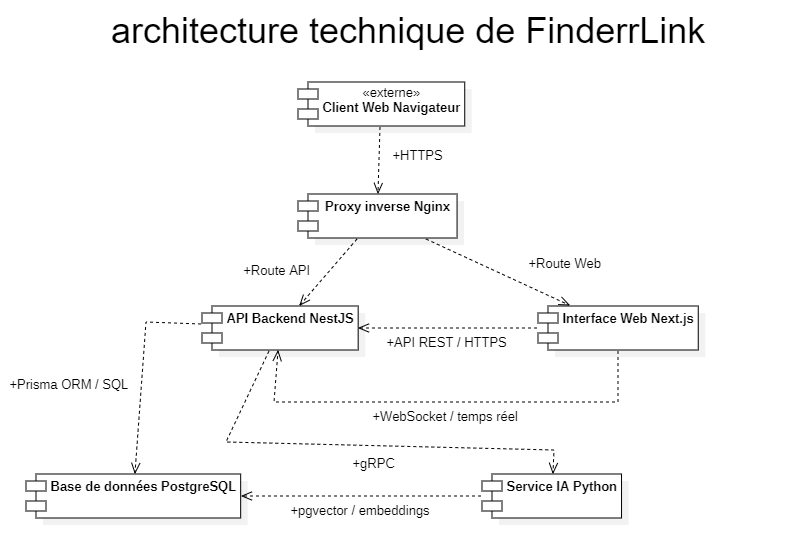
\includegraphics[width=0.95\textwidth]{./figures/ComponentDiagram1.png}
\caption{Diagramme de composants - FinderrLink}
\label{fig:component_diagram_finderrlink}
\end{figure}

\subsection{Explication du diagramme de composants}

Le client web navigateur represente l'utilisateur qui accede a la plateforme depuis un navigateur. Toutes les requetes passent d'abord par le proxy inverse Nginx, qui joue le role d'intermediaire entre l'utilisateur et les services internes.

L'interface web Next.js represente la partie frontend de l'application. Elle est responsable de l'affichage des pages, de l'experience utilisateur et de l'interaction avec les differents profils. L'API Backend NestJS represente la partie serveur. Elle contient la logique metier, la gestion des utilisateurs, des missions, des candidatures, des notifications et des communications avec les autres services.

La base de donnees PostgreSQL assure la persistance des donnees. Elle stocke les utilisateurs, les profils, les missions, les candidatures, les messages et les notifications. Le service IA Python represente le microservice intelligent utilise par FinderrLink pour traiter les demandes liees a l'assistant IA, comme la recherche de missions adaptees, la recommandation de talents ou la generation de reponses.

Ce diagramme montre que FinderrLink est organise selon une architecture separee en plusieurs composants. Cette separation facilite la maintenance, le deploiement, l'evolutivite et l'integration future de nouveaux services.
\section{Diagramme d'activite du service IA}

Le diagramme d'activite suivant presente le fonctionnement general du service d'intelligence artificielle integre dans FinderrLink. Ce diagramme permet de comprendre comment une demande utilisateur est analysee, filtree, traitee puis transformee en reponse avant d'etre retournee au backend de l'application.

\begin{landscape}
\begin{figure}[H]
\centering
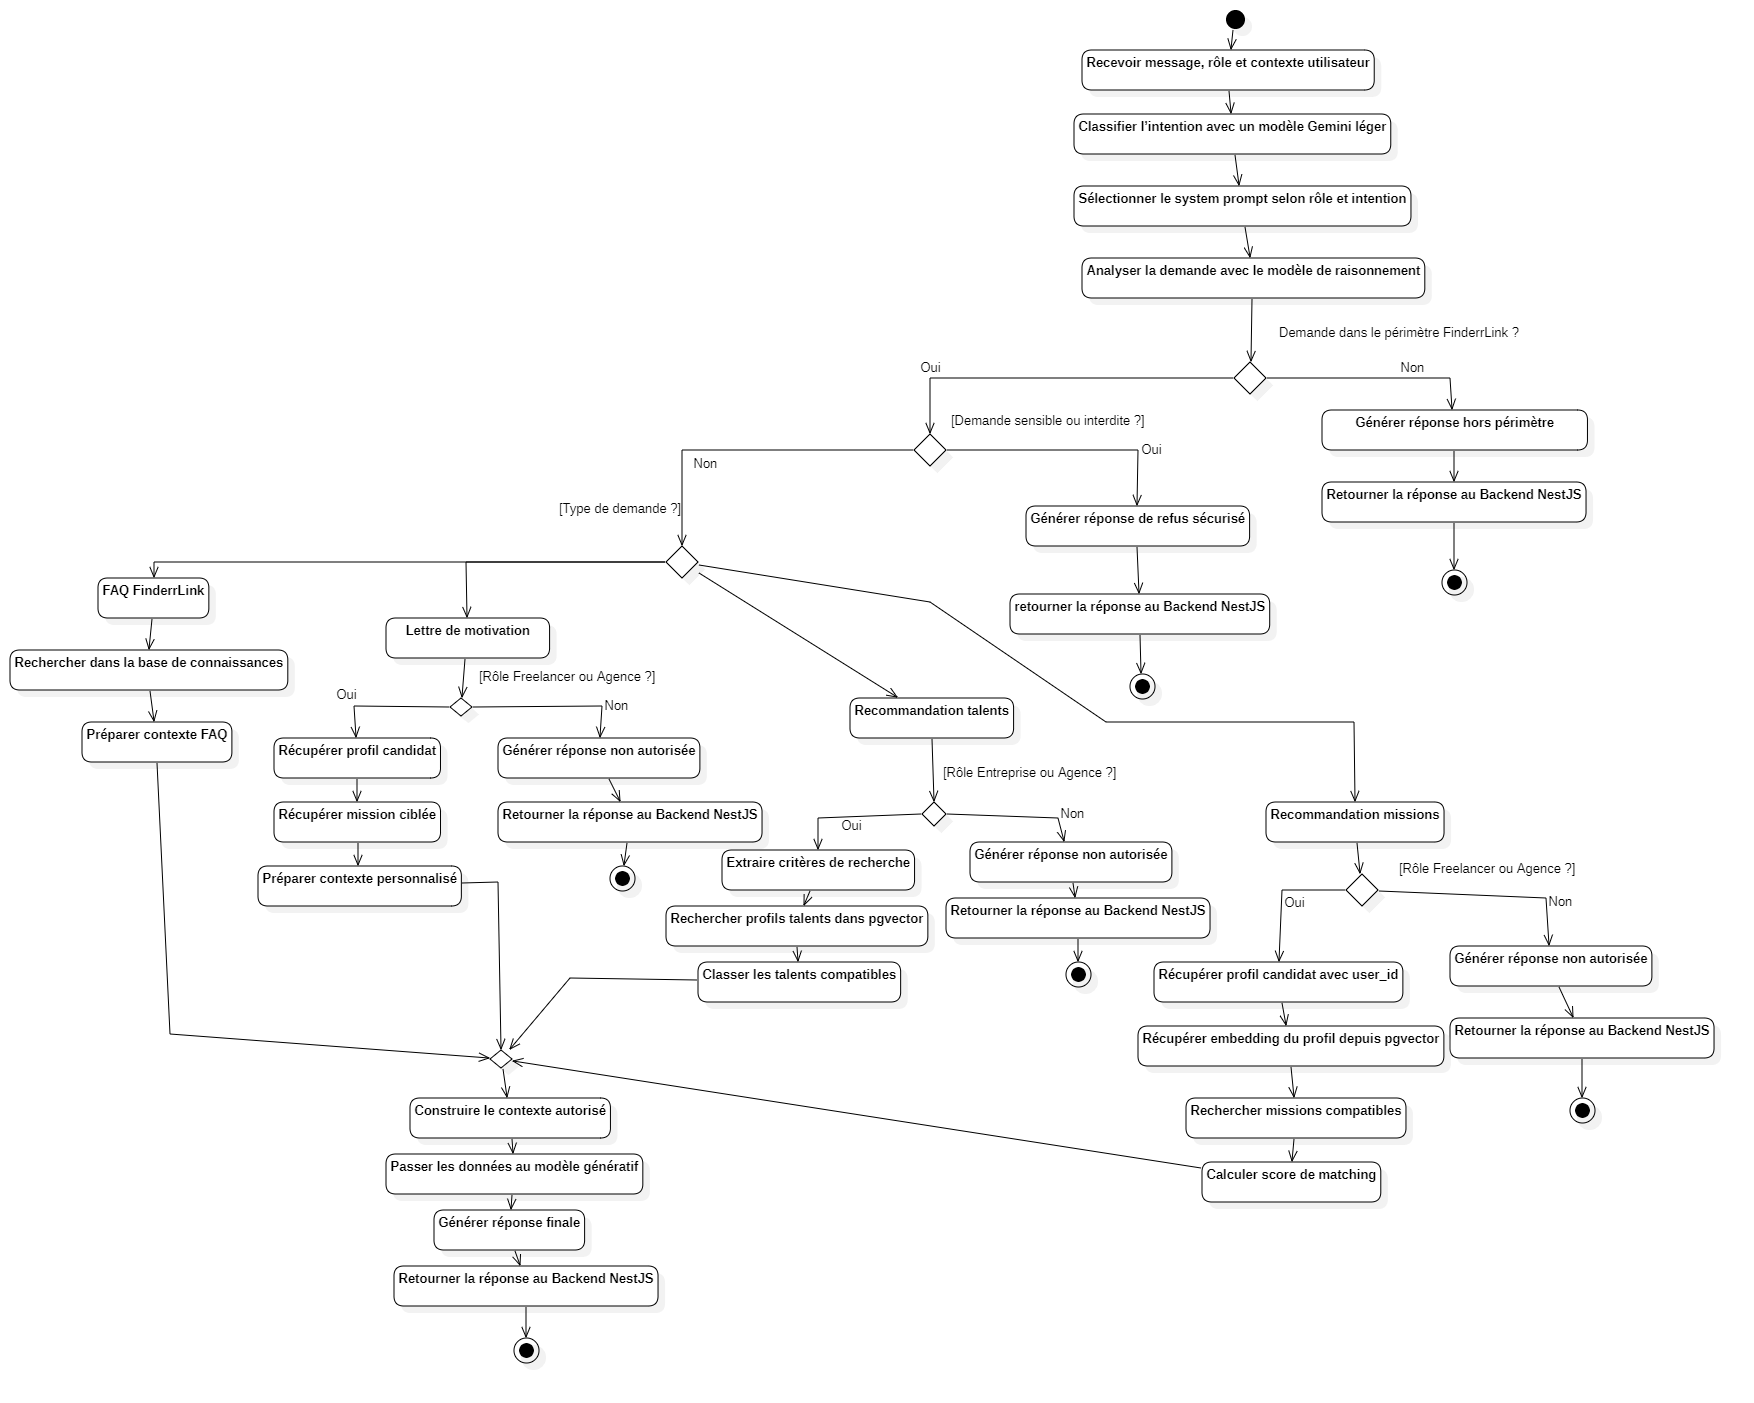
\includegraphics[width=0.95\linewidth]{./figures/ActivityDiagram1.png}
\caption{Diagramme d'activite du service IA - FinderrLink}
\label{fig:activity_diagram_ai_finderrlink}
\end{figure}
\end{landscape}

\subsection{Explication du diagramme d'activite IA}

Le processus commence par la reception du message de l'utilisateur avec son role et son contexte. Ces informations sont importantes, car les reponses de l'assistant doivent respecter les droits de chaque type d'utilisateur. Par exemple, un freelance ne doit pas acceder aux memes informations qu'une entreprise ou qu'une agence.

La premiere etape consiste a classifier l'intention de la demande a l'aide d'un modele Gemini leger. Cette classification permet d'identifier le type de besoin exprime par l'utilisateur, comme une recherche de missions, une recommandation de talents, une generation de lettre de motivation ou une question FAQ. Ensuite, le systeme selectionne le system prompt adapte au role et a l'intention afin d'encadrer correctement la reponse de l'assistant.

Apres cette premiere analyse, la demande est transmise a un modele de raisonnement plus avance. Ce modele verifie si la demande entre dans le perimetre de FinderrLink et si elle respecte les regles de securite. Si la demande est hors perimetre, le systeme genere une reponse adaptee sans acceder aux donnees internes. Si la demande est interdite ou non autorisee, une reponse de refus securisee est retournee.

Lorsque la demande est valide, le systeme suit un traitement specifique selon son type. Pour une recommandation de missions, le service recupere le profil du candidat, recherche les missions compatibles dans la base vectorielle et calcule un score de matching. Pour une recommandation de talents, il extrait les criteres de recherche, interroge les profils disponibles et classe les talents compatibles. Pour une lettre de motivation, il recupere le profil du candidat et la mission ciblee afin de construire un contexte personnalise. Pour une question FAQ, il recherche la reponse dans la base de connaissances de FinderrLink.

Enfin, les donnees autorisees sont transmises au modele generatif afin de produire une reponse finale claire et adaptee. Cette reponse est ensuite retournee au backend NestJS, qui se charge de l'envoyer a l'interface utilisateur. Ce fonctionnement montre que le service IA de FinderrLink ne se limite pas a generer du texte : il applique aussi une logique de classification, de controle d'acces, de recherche contextuelle et de generation securisee.

\section{Conclusion}

Cette conception permet de mieux comprendre l'organisation generale de FinderrLink. Le diagramme de cas d'utilisation montre les principales interactions entre les acteurs et la plateforme. Le diagramme de classes presente la structure interne du systeme. Le diagramme de composants montre l'architecture technique globale, composee du client web, du proxy Nginx, du frontend Next.js, du backend NestJS, de la base de donnees PostgreSQL et du service IA Python.


\newpage

\markboth{\MakeUppercase{Réalisation de l'Application}}{}
\chapter{ Mise en œuvre et Évolution}
\markboth{\MakeUppercase{CHAPITRE 5. Mise en œuvre et Évolution}}{}

\section{Introduction Générale}

Le développement de l'application \textbf{Mediassive Analytics} représente une approche moderne et intégrée, combinant les meilleures pratiques du développement web contemporain avec des technologies de pointe. Cette solution SaaS innovante a été conçue pour répondre aux besoins spécifiques d'une agence de marketing digital, en offrant une plateforme centralisée d'analyse et de suivi des performances marketing.

L'architecture technique adoptée suit les principes du développement full-stack moderne, avec une séparation claire entre le frontend et le backend, une base de données robuste, et des intégrations API avancées. Cette approche garantit non seulement la performance et la scalabilité de l'application, mais aussi sa maintenabilité et son évolutivité future.

Le projet s'inscrit dans une démarche d'excellence technique, utilisant des frameworks et outils reconnus dans l'industrie, tout en intégrant des fonctionnalités innovantes comme la section \textit{Web3 Trends} qui positionne l'application à l'avant-garde des technologies émergentes.

\section{Technologies Utilisées}

\subsection{Frontend}

\begin{figure}[H]
\centering

\includegraphics[width=0.4\textwidth]{figures/tech/nextjs.png}\\[0.3cm]
Next.js est un framework basé sur React qui permet le rendu côté serveur (SSR) et des optimisations automatiques\cite{nextjs}. Il a été utilisé pour développer l’interface utilisateur moderne et performante de l’application.
\caption{Next.js}
\end{figure}

\begin{figure}[H]
\centering

\includegraphics[width=0.4\textwidth]{figures/tech/tailwind.png}\\[0.3cm]
Tailwind CSS est un framework CSS utilitaire pour construire rapidement des interfaces modernes et responsive\cite{tailwind}. Il a été utilisé pour styliser l’application de manière cohérente et efficace.
\caption{Tailwind CSS}
\end{figure}

\begin{figure}[H]
\centering

\includegraphics[width=0.4\textwidth]{figures/tech/chart.js.png}\\[0.3cm]
Chart.js est une bibliothèque de visualisation de données interactive\cite{chartjs}. Elle a été utilisée pour afficher des graphiques et tableaux de bord dynamiques et performants.
\caption{Chart.js}
\end{figure}

\subsection{Backend}

\begin{figure}[H]
\centering

\includegraphics[width=0.4\textwidth]{figures/tech/nestjs.jpeg}\\[0.3cm]
NestJS est un framework Node.js pour créer des applications backend scalables et maintenables\cite{nestjs}. Il a été utilisé pour gérer la logique métier, les APIs et la communication avec la base de données.
\caption{NestJS}
\end{figure}

\begin{figure}[H]
\centering

\includegraphics[width=0.4\textwidth]{figures/tech/supabase.png}\\[0.3cm]
Supabase est une plateforme backend-as-a-service basée sur PostgreSQL\cite{supabase,postgresql}. Elle a été utilisée pour héberger la base de données et gérer l’authentification et le stockage.
\caption{Supabase}
\end{figure}

\subsection{Outils de Développement}

\begin{figure}[H]
\centering

\includegraphics[width=0.4\textwidth]{figures/tech/vscode.png}\\[0.3cm]
Visual Studio Code est un éditeur de code moderne avec de nombreuses extensions. Il a été utilisé pour développer l’ensemble de l’application de manière productive et organisée.
\caption{VS Code}
\end{figure}

\begin{figure}[H]
\centering

\includegraphics[width=0.4\textwidth]{figures/tech/googleanal.png}\\[0.3cm]
Google Analytics permet de suivre le trafic web et les conversions\cite{ga4}. Il a été intégré pour analyser les performances marketing de l’application.
\caption{Google Analytics}
\end{figure}

\begin{figure}[H]
\centering

\includegraphics[width=0.4\textwidth]{figures/tech/metadev.png}\\[0.3cm]
Meta for Developers fournit des APIs pour Facebook et Instagram\cite{meta}. Elles ont été utilisées pour récupérer les données sociales et intégrer les statistiques dans l’application.
\caption{Meta for Developers}
\end{figure}

\begin{figure}[H]
\centering

\includegraphics[width=0.4\textwidth]{figures/tech/google.png}\\[0.3cm]
Google Cloud fournit des services d’infrastructure et de plateforme (IaaS/PaaS) pour l’hébergement, le stockage et l’orchestration à grande échelle\cite{gcp}. Il permet aussi de gérer et d’exposer des APIs (API Gateway, Cloud Endpoints) et de sécuriser l’accès/connexion aux services (IAM, OAuth2), afin de contrôler l’authentification et les autorisations au niveau de l’application.
\caption{Google Cloud}
\end{figure}

\section{Architecture Technique}

L'architecture de Mediassive Analytics repose sur une approche moderne et évolutive, organisée en plusieurs couches distinctes :

\begin{itemize}
    \item \textbf{Frontend} : Interface utilisateur moderne développée avec Next.js et Tailwind CSS
    \item \textbf{Backend} : API REST robuste construite avec NestJS et Node.js
    \item \textbf{Base de données} : PostgreSQL\cite{postgresql} hébergé sur Supabase\cite{supabase} avec Prisma ORM\cite{prisma}
    \item \textbf{Intégrations} : APIs tierces (Google Analytics\cite{ga4}, Meta\cite{meta}, LinkedIn\cite{linkedin}) pour la collecte de données
    \item \textbf{Visualisation} : Chart.js pour les graphiques et tableaux de bord interactifs
\end{itemize}

Cette architecture garantit une séparation claire des responsabilités, une maintenance facilitée et une scalabilité optimale pour répondre aux besoins croissants de l'application.
\section{Rapidité et optimisation}

L'application peut traiter 5 000 à 10 000 enregistrements en moins de 3 secondes grâce à Next.js côté front-end et PostgreSQL côté base de données. L'optimisation des requêtes SQL via Prisma et l'utilisation de cache (ISR) assurent une navigation fluide.

\section{Stabilité et sécurité}

Des tests unitaires (Jest) et d'intégration (Cypress) garantissent la fiabilité des fonctionnalités critiques. La sécurité est renforcée par NextAuth.js, la gestion des rôles et le chiffrement SSL des échanges de données.

\section{Expérience utilisateur}

L'interface est intuitive, rapide et responsive, utilisant Tailwind CSS et Framer Motion pour une navigation agréable, même sur mobile.

\section{Améliorations futures}

\subsection{Optimisation technique}

Prévoir un cache plus avancé (Redis), l'analyse de volumes plus importants via un Data Lake (BigQuery) et un monitoring temps réel (Grafana, Prometheus).

\subsection{Intelligence Artificielle}

Intégrer un module IA capable d’analyser les données marketing, détecter des anomalies dans les KPI et produire des prédictions pour optimiser les campagnes publicitaires.

\subsection{Personnalisation et API}

Permettre la personnalisation des rapports avec des widgets dynamiques et proposer une API publique pour intégrer Mediassive Analytics dans les systèmes clients.
\newpage

\markboth{\MakeUppercase{Évaluation et Perspectives}}{}
\chapter{Évaluation et Perspectives}
\section*{Résumé du chapitre}

Ce chapitre présente l'évaluation de FinderrLink à travers des tests manuels, des vérifications backend, des essais sur l'assistant IA et un test de charge avec k6. Il analyse les limites actuelles de performance et propose des pistes d'optimisation. Il présente enfin les perspectives d'évolution comme la visioconférence, le multilingue, l'IA agentique et l'application mobile.

\section{Introduction}

Ce chapitre présente l'évaluation de la plateforme FinderrLink après sa réalisation et son déploiement. L'objectif est de vérifier le bon fonctionnement général de l'application, d'analyser les premiers résultats de performance et d'identifier les améliorations possibles pour les prochaines versions.

L'évaluation réalisée repose principalement sur des tests fonctionnels manuels, des vérifications backend, des essais de sécurité sur l'assistant IA et un test de charge réalisé avec l'outil \texttt{k6} \cite{k6}. Ces tests ne représentent pas une campagne complète de validation industrielle, mais ils permettent d'avoir une première vision de la stabilité de la plateforme et de ses limites actuelles.

\section{Validation fonctionnelle de l'interface utilisateur}

La première étape de validation a concerné l'interface utilisateur de FinderrLink. Les tests ont été réalisés manuellement sur les principales pages de la plateforme afin de vérifier que les parcours utilisateurs fonctionnent correctement.

Les pages communes ont été testées, notamment la page d'accueil, l'inscription, la connexion, la récupération du mot de passe, les notifications et l'historique de l'assistant IA. Les espaces spécifiques aux rôles ont également été vérifiés : espace Freelance, espace Entreprise, espace Agence et espace Administration.

Dans l'espace Freelance, les vérifications ont porté sur la recherche de missions, le détail d'une mission, la soumission d'une candidature, le suivi des candidatures, la messagerie et la gestion du profil. Dans l'espace Entreprise, les tests ont concerné la gestion des missions, la consultation des candidatures reçues, la recherche de freelances et la messagerie. Dans l'espace Agence, les tests ont permis de vérifier le comportement hybride du rôle, c'est-à-dire la possibilité de publier des missions et de postuler à des missions disponibles.

Globalement, les parcours principaux testés manuellement ont fonctionné correctement. Les anomalies détectées durant cette phase ont été corrigées progressivement afin d'améliorer la cohérence de l'interface et la fluidité de l'utilisation.

\section{Validation du backend}

La validation backend a porté sur les principales fonctionnalités exposées par l'API de FinderrLink. Les vérifications ont concerné l'authentification, la gestion des rôles, les missions, les candidatures, les profils, les notifications, la messagerie et la communication avec les autres services.

Les tests ont permis de vérifier que les données étaient correctement échangées entre l'interface frontend, l'API backend et la base de données PostgreSQL \cite{postgresql}. Les principales routes utilisées par l'application ont été validées à travers les parcours utilisateurs réels.

Une attention particulière a été accordée au système RBAC, car FinderrLink repose sur plusieurs rôles : Freelance, Entreprise, Agence et Administrateur. Les vérifications ont montré que les fonctionnalités accessibles changent bien selon le rôle de l'utilisateur. Le rôle Agence a également été vérifié, car il combine certaines permissions du Freelance et certaines permissions de l'Entreprise.

\section{Validation de l'assistant IA et sécurité des prompts}

L'assistant IA de FinderrLink a été testé à travers plusieurs prompts liés aux usages principaux de la plateforme. Les tests ont concerné la recommandation de missions pour les freelances, la recommandation de profils pour les entreprises, l'aide à la rédaction de messages et les réponses aux questions générales sur la plateforme.

Des essais de prompt injection ont également été réalisés afin de vérifier que l'assistant ne fournit pas d'informations non autorisées et qu'il reste dans le périmètre fonctionnel de FinderrLink. Les tests effectués ont montré que l'assistant respecte le rôle de l'utilisateur et refuse les demandes qui sortent du cadre autorisé.

Cette validation reste toutefois une première étape. Pour une version plus avancée, il sera nécessaire de réaliser une campagne plus large de tests IA avec différents scénarios, plusieurs langues, des cas limites et des tentatives d'injection plus variées.

\section{Test de charge avec k6}

Afin d'évaluer la capacité de la plateforme à supporter un volume important de requêtes, un test de charge a été réalisé avec l'outil \texttt{k6} \cite{k6}. Le test a été exécuté depuis mon ordinateur personnel et non directement depuis le VPS. Comme le DNS Docker ne fonctionnait pas normalement sous Arch Linux, l'exécution a été réalisée avec l'option \texttt{--network host} \cite{docker}.

\begin{verbatim}
docker run --rm --network host -i grafana/k6 run - < limit-test.js
\end{verbatim}

Plusieurs outils ont été utilisés pendant cette phase de test :

\begin{itemize}
\item \texttt{curl} pour vérifier que le domaine répond correctement.
\item \texttt{docker stats} pour surveiller les conteneurs sur le VPS.
\item \texttt{htop} pour surveiller l'utilisation CPU et RAM.
\item Les logs Nginx pour vérifier les erreurs et les timeouts.
\item Les seuils k6 pour mesurer les échecs, le temps de réponse p95 et les itérations abandonnées.
\end{itemize}

L'URL principalement testée était :

\begin{center}
\texttt{https://app.finderrlink.com/login}
\end{center}

\section{Résultats du test de charge}

Le premier test a simulé 400 utilisateurs virtuels sur la page de connexion frontend.

\begin{table}[H]
\centering
\small
\renewcommand{\arraystretch}{1.3}
\begin{tabular}{|p{6cm}|p{6cm}|}
\hline
\textbf{Indicateur} & \textbf{Résultat} \\
\hline
Nombre maximal d'utilisateurs virtuels & 400 \\
\hline
Nombre total de requêtes & 43,029 \\
\hline
Débit moyen & Environ 102 requêtes/seconde \\
\hline
Requêtes échouées & 0\% \\
\hline
Temps de réponse p95 & 132 ms \\
\hline
Utilisation CPU & Environ 20--30\% \\
\hline
Utilisation RAM & Environ 3\% \\
\hline
Résultat & Test réussi \\
\hline
\end{tabular}
\caption{Résultat du test avec 400 utilisateurs virtuels sur la page de connexion}
\label{tab:k6-vu-login}
\end{table}

Ce premier test montre que la page frontend de connexion a supporté 400 utilisateurs virtuels sans échec. Les temps de réponse sont restés faibles et l'utilisation des ressources serveur est restée acceptable.

Ensuite, des tests à débit fixe ont été réalisés afin d'identifier la capacité stable de la page.

\begin{table}[H]
\centering
\small
\renewcommand{\arraystretch}{1.3}
\begin{tabular}{|p{3cm}|p{3cm}|p{3cm}|p{3cm}|p{2cm}|}
\hline
\textbf{Débit ciblé} & \textbf{Requêtes totales} & \textbf{Échecs} & \textbf{p95} & \textbf{Résultat} \\
\hline
100 RPS & 12,000 & 0,80\% & 87,24 ms & Réussi \\
\hline
200 RPS & 24,001 & 0,63\% & 103,55 ms & Réussi \\
\hline
400 RPS & 47,411 & 2,71\% & 373,47 ms & Zone de stress \\
\hline
\end{tabular}
\caption{Résultats des tests à débit fixe avec k6}
\label{tab:k6-fixed-rate}
\end{table}

À 100 requêtes par seconde, la plateforme a atteint un débit réel de 99,93 RPS sans itérations abandonnées. À 200 requêtes par seconde, le débit réel a atteint 199,87 RPS, avec un taux d'échec limité et aucun abandon d'itération. Ces deux niveaux sont considérés comme stables pour la page testée.

À 400 requêtes par seconde, le débit réel a atteint environ 380,38 RPS. Le serveur a continué à répondre, mais 590 itérations ont été abandonnées et le taux d'échec est monté à 2,71%. Le temps de réponse p95 est resté inférieur à 400 ms, mais le temps maximal a atteint 5,38 secondes. Ce résultat indique que le système commence à atteindre une zone de stress à ce niveau de charge.

\section{Analyse des résultats}

Les résultats montrent que la capacité stable confirmée de la page frontend de connexion se situe autour de 200 requêtes par seconde. À ce niveau, le système répond correctement, sans itérations abandonnées et avec un temps de réponse p95 inférieur à 110 ms.

À partir de 400 requêtes par seconde, la plateforme commence à montrer des signes de limite : apparition d'itérations abandonnées, augmentation du taux d'échec et hausse du temps de réponse maximal. Le serveur continue de répondre, mais cette charge ne doit pas être considérée comme stable pour une utilisation continue.

Il est important de préciser que ce test concerne principalement la page frontend de connexion. Il ne représente pas la capacité complète de l'application avec toutes ses fonctionnalités : tableau de bord, authentification réelle, base de données, messagerie, service IA, routes protégées et traitement des candidatures.

Lors d'un test direct sur l'endpoint réel de connexion \texttt{POST /api/auth/login}, le backend a retourné le statut \texttt{429 Too Many Requests}. Ce comportement montre que le rate limiter du backend fonctionne correctement. Par conséquent, cet endpoint ne peut pas être utilisé directement pour mesurer la capacité brute du serveur, sauf dans un environnement de staging avec des limites temporairement ajustées.

\section{Limites de l'évaluation}

L'évaluation réalisée présente plusieurs limites. Les tests fonctionnels ont été réalisés manuellement et ne remplacent pas des tests automatisés complets. Les tests backend ont validé les principaux parcours, mais ils ne couvrent pas encore tous les cas limites possibles.

Le test k6 a principalement mesuré la capacité de la page frontend de connexion. Il ne mesure pas encore la charge réelle sur les routes protégées, les requêtes avec base de données, la messagerie WebSocket, le service IA ou les traitements complexes de candidatures.

Enfin, les tests de sécurité de l'assistant IA et les essais de prompt injection ont été réalisés sur des scénarios limités. Ils confirment un premier niveau de protection, mais une validation plus poussée reste nécessaire pour une version de production avancée.

\section{Seuils de montée en charge et décision d'évolution}

D'après les premiers résultats, la plateforme peut être considérée comme stable pour la page testée jusqu'à environ 200 requêtes par seconde. Si FinderrLink atteint une utilisation réelle proche de ce niveau de manière régulière, il sera nécessaire de prévoir une évolution de l'infrastructure.

Une première décision d'amélioration doit être envisagée si l'un des seuils suivants est atteint :

\begin{itemize}
\item plus de 150 à 200 requêtes par seconde de manière régulière ;
\item un temps de réponse p95 supérieur à 500 ms pendant plusieurs minutes ;
\item un taux d'erreur supérieur à 1% sur les pages ou routes principales ;
\item une utilisation CPU supérieure à 70% de manière continue ;
\item une utilisation RAM supérieure à 75% de manière continue ;
\item des ralentissements visibles sur les pages protégées ou la messagerie.
\end{itemize}

Dans ce cas, il sera préférable d'acheter un VPS dédié uniquement à FinderrLink, avec de meilleures ressources CPU, RAM et stockage. Cette séparation permettra d'éviter que d'autres projets ou services hébergés sur le même serveur influencent les performances de la plateforme.

\section{Optimisations techniques proposées}

Plusieurs pistes d'optimisation peuvent être mises en place pour améliorer les performances de FinderrLink.

La première consiste à optimiser le frontend Next.js, notamment en réduisant la taille des bundles, en optimisant les images, en utilisant le caching et en évitant les chargements inutiles de données. Les pages les plus consultées, comme la landing page, la connexion et les tableaux de bord, doivent être particulièrement optimisées.

La deuxième piste concerne le backend NestJS \cite{nestjs}. Il est possible d'améliorer les requêtes vers la base de données, d'ajouter des index PostgreSQL sur les champs fréquemment utilisés, de mettre en cache certaines données et de réduire les traitements répétitifs \cite{postgresql}. Les endpoints sensibles doivent garder un rate limiting adapté afin de protéger l'application.

La troisième piste concerne la base de données. PostgreSQL peut être optimisé à travers l'ajout d'index, l'analyse des requêtes lentes, la séparation éventuelle des lectures et écritures, ainsi que la surveillance de la latence. Pour les fonctionnalités IA utilisant des embeddings, l'optimisation de pgvector peut également améliorer les temps de réponse \cite{pgvector}.

La quatrième piste concerne l'infrastructure. À moyen terme, FinderrLink pourra évoluer vers une architecture plus scalable avec un load balancer, plusieurs instances backend, un service IA isolé et une base de données mieux dimensionnée. Cette évolution permettra de mieux absorber l'augmentation du nombre d'utilisateurs.

\section{Perspectives d'architecture}

Dans la version actuelle, FinderrLink repose sur une architecture modulaire avec un frontend, un backend, une base de données, un service IA et un proxy Nginx. Cette organisation est suffisante pour une première version fonctionnelle et déployée.

Cependant, si la plateforme atteint un volume important d'utilisateurs, une évolution vers une architecture plus avancée sera nécessaire. Le backend pourra être progressivement découpé en microservices selon les domaines fonctionnels : authentification, missions, candidatures, messagerie, notifications, administration et intelligence artificielle.

Un load balancer pourra être ajouté afin de répartir le trafic entre plusieurs instances backend. La messagerie en temps réel pourra être isolée dans un service dédié, afin de mieux gérer les connexions WebSocket. Le service IA pourra également être déployé sur une machine séparée, avec plus de ressources si les traitements deviennent plus lourds.

Cette évolution permettra d'améliorer la disponibilité, la performance et la maintenabilité de la plateforme. Elle devra toutefois être réalisée progressivement, car une architecture microservices ajoute aussi plus de complexité au niveau du déploiement, de la supervision et de la communication entre services.

\section{Perspectives fonctionnelles}

Plusieurs améliorations fonctionnelles sont prévues pour les prochaines versions de FinderrLink. La première perspective concerne l'ajout d'un système de visioconférence intégré. Cette fonctionnalité permettra aux entreprises, agences et freelances d'organiser des entretiens directement depuis la plateforme, sans passer par des outils externes.

La deuxième perspective concerne le support multilingue. FinderrLink pourra proposer une interface en plusieurs langues afin de faciliter son utilisation par des profils internationaux. Cette évolution concerne à la fois l'interface, les messages système, les notifications et l'assistant IA.

La troisième perspective concerne l'amélioration de l'assistant IA vers une approche plus agentique. L'objectif serait de permettre à l'IA d'accompagner davantage l'utilisateur dans des actions complexes, comme comparer plusieurs profils, préparer une shortlist, suggérer des améliorations de profil ou aider à planifier un processus de recrutement.

Enfin, une application mobile native pourra être développée afin d'améliorer l'accessibilité de la plateforme. Cette application permettrait aux utilisateurs de consulter les missions, suivre les candidatures, recevoir des notifications et échanger par messagerie directement depuis un smartphone.

\section{Conclusion}

Cette évaluation a permis de vérifier le bon fonctionnement général de FinderrLink à travers des tests manuels, des validations backend, des essais sur l'assistant IA et un test de charge avec k6. Les résultats montrent que la plateforme fonctionne correctement dans son état actuel et que la page frontend de connexion supporte une charge stable jusqu'à environ 200 requêtes par seconde.

Les tests ont également montré que la plateforme commence à atteindre une zone de stress autour de 400 requêtes par seconde pour la page testée. Cette limite ne représente pas toute l'application, mais elle donne une première indication utile pour préparer l'évolution de l'infrastructure.

Les prochaines améliorations devront porter sur l'automatisation des tests, l'optimisation des performances, l'amélioration de la sécurité IA, la montée en charge de l'infrastructure et l'ajout de nouvelles fonctionnalités comme la visioconférence, le multilingue, l'IA agentique et l'application mobile native.

\newpage
\markboth{\MakeUppercase{Conclusion Générale}}{}
\addcontentsline{toc}{chapter}{Conclusion Générale}
\chapter*{Conclusion générale}
\addcontentsline{toc}{chapter}{Conclusion générale}
\markboth{\MakeUppercase{Conclusion générale}}{}

Ce Projet de Fin d'Études réalisé au sein de MEDIASSIVE m'a permis de participer à la conception, au développement, au déploiement et à l'évaluation de FinderrLink, une plateforme SaaS facilitant la mise en relation entre freelances, entreprises et agences, avec une centralisation des profils, missions, candidatures, échanges et notifications dans un environnement unique et sécurisé.

Durant cette mission, j'ai occupé le rôle de chef d'équipe stagiaire, développeur full-stack et responsable du déploiement, couvrant le développement frontend et backend, l'intégration des services, la coordination de l'équipe et la mise en ligne de la plateforme. Cette expérience m'a permis d'évoluer dans un contexte proche d'un environnement professionnel réel, avec des contraintes techniques, organisationnelles et humaines.

FinderrLink repose sur quatre rôles principaux — Freelance, Entreprise, Agence et Administrateur — chacun disposant de fonctionnalités adaptées via un système RBAC. La plateforme couvre la gestion des profils, la publication et recherche de missions, le suivi des candidatures, la messagerie, les notifications et un assistant intelligent. L'agence se distingue par son rôle hybride, lui permettant à la fois de publier des missions et de postuler à des opportunités.

Sur le plan technique, la solution s'appuie sur une architecture full-stack moderne : frontend Next.js, backend NestJS, base de données PostgreSQL, service IA en Python, et un déploiement via Docker, Nginx et VPS. Cette architecture garantit une séparation claire des responsabilités et prépare la plateforme à une évolution future.

La phase d'évaluation, menée à travers des tests manuels, des validations backend et un test de charge k6, confirme le bon fonctionnement général de FinderrLink tout en identifiant des pistes d'amélioration. Ce stage a renforcé mes compétences en développement web, déploiement et gestion de projet. FinderrLink reste une plateforme évolutive, avec des perspectives incluant les tests automatisés, la visioconférence, le support multilingue, l'IA agentique et une application mobile native.




\chapter*{Bibliographie}

\begin{thebibliography}{99}

[1] Next.js Documentation, [En ligne]. Disponible sur :
https://nextjs.org/docs (Consulté le : 2026-01-15).

[2] Tailwind CSS Documentation, [En ligne]. Disponible sur :
https://tailwindcss.com/docs (Consulté le : 2026-01-15).

[3] NestJS Documentation, [En ligne]. Disponible sur :
https://docs.nestjs.com/ (Consulté le : 2026-01-15).

[4] Prisma ORM Documentation, [En ligne]. Disponible sur :
https://www.prisma.io/docs (Consulté le : 2026-01-20).

[5] PostgreSQL Documentation, [En ligne]. Disponible sur :
https://www.postgresql.org/docs/ (Consulté le : 2026-01-20).

[6] pgvector GitHub Repository, [En ligne]. Disponible sur :
https://github.com/pgvector/pgvector (Consulté le : 2026-02-01).

[7] JSON Web Tokens — Introduction, [En ligne]. Disponible sur :
https://jwt.io/introduction (Consulté le : 2026-01-10).

[8] OWASP Top Ten 2021, [En ligne]. Disponible sur :
https://owasp.org/www-project-top-ten/ (Consulté le : 2026-01-10).

[9] Socket.IO Documentation, [En ligne]. Disponible sur :
https://socket.io/docs/v4/ (Consulté le : 2026-01-25).

[10] Nodemailer Documentation, [En ligne]. Disponible sur :
https://nodemailer.com/about/ (Consulté le : 2026-02-05).

[11] Handlebars.js Documentation, [En ligne]. Disponible sur :
https://handlebarsjs.com/guide/ (Consulté le : 2026-02-05).

[12] Google Gemini API Documentation, [En ligne]. Disponible sur :
https://ai.google.dev/gemini-api/docs (Consulté le : 2026-02-10).

[13] FastAPI Documentation, [En ligne]. Disponible sur :
https://fastapi.tiangolo.com/ (Consulté le : 2026-01-18).

[14] Ollama GitHub Repository, [En ligne]. Disponible sur :
https://github.com/ollama/ollama (Consulté le : 2026-02-10).

[15] gRPC Documentation, [En ligne]. Disponible sur :
https://grpc.io/docs/ (Consulté le : 2026-01-22).

[16] Docker Documentation, [En ligne]. Disponible sur :
https://docs.docker.com/ (Consulté le : 2026-02-15).

[17] Nginx Documentation, [En ligne]. Disponible sur :
https://nginx.org/en/docs/ (Consulté le : 2026-02-15).

[18] Certbot Documentation, [En ligne]. Disponible sur :
https://certbot.eff.org/docs/ (Consulté le : 2026-02-15).

[19] GitHub Actions Documentation, [En ligne]. Disponible sur :
https://docs.github.com/en/actions (Consulté le : 2026-03-01).

[20] Grafana k6 Documentation, [En ligne]. Disponible sur :
https://grafana.com/docs/k6/latest/ (Consulté le : 2026-03-10).

[21] TypeScript Documentation, [En ligne]. Disponible sur :
https://www.typescriptlang.org/docs/ (Consulté le : 2026-01-08).

[22] Figma Help Center, [En ligne]. Disponible sur :
https://help.figma.com/ (Consulté le : 2026-01-08).

[23] Object Management Group, Unified Modeling Language (UML)
Version 2.5.1, 2017. Disponible sur :
https://www.omg.org/spec/UML/2.5.1/ (Consulté le : 2026-01-05).
\addcontentsline{toc}{chapter}{Références Bibliographiques}

\end{document}
